\chapter{Uvod}

Digitalna tehnologija obuhaća gotovo sve aspekte ljudskog života, od komunikacije, poslovanja do zabave i znanja. Rekreativne aktivnosti i sportovi koji su se oslanjali na fizičku opremu i materijale sve više usvajaju digitalne alate koji proširuju mogućnosti i količinu informacija koje korisnici mogu dobiti. Sportsko penjanje, kao aktivnost koja spaja fizičku spremnost i boravak u prirodi, predstavlja primjer aktivnosti koja se može proširiti digitalnim alatima.

Dok su postojeće digitalne platforme omogućile lak pristup informacijama penjačkih lokacija, ključni izazov ostaje upotreba tih informacija u stvarnom okruženju - isprijed same stijene. Taj ključni izazov otvara prostor za inovacije, posebice u domeni mobilnih tehnologija, računalnog vida i proširene stvarnosti.

\section{Kontekst i rast popularnosti sportskog penjanja} 

Sportsko penjanje i srodna disciplina \textit{bouldering} posljednjih su desetljeća doživjeli eksponencijalni rast u popularnosti, Privlačeći sve veći broj zainteresiranih ljudi kako u specijalizirane penjačke dvorane, tako i na prirodne stijene. Na Olimpijskim igrama 2020. godine u Tokiju sportsko penjanje je po prvi put uvršten u program čime je sport dobio globalnu pozornost i dodatno potaknuo interes javnosti. Olimpijskim igrama 2024. godine u Parizu popularnost sporta je još više porasla. Prema članku iz \textit{The Oxford Blue}, dok se vrijednost globalnog tržišta penjačkih dvorana procjenjuje na 117.61 milijardi dolara do 2031. godine \cite{the_oxford_blue_rock_climb}. S rastom zajednice, raste i potreba za kvalitetnim, dostupnim i preciznim informacijama o penjalištima i smjerovima. 
\section{Problem identifikacije penjačkih smjerova i ograničenja tradictionalnih alata}

Tradicionalno, glavni izvor informacija za penjače su tiskani penjački vodiči. Ovi vodiči sadrže detaljne opise penjačkih lokacija, karte pristupa, kao i skicirane prikaze stijene ili često nazivane \textit{topo} s ocrtanim linijama penjačkih smjerova, njihovim nazivima i težinama. Iako su desetljećima bili nezamjenjiv alat, tiskani vodiči imaju ograničenja. 
Podložni su zastarijevanju jer ne mogu pratiti dinamiku promjena na penjačkim lokacijama poput dodavanja novih smjerova, promjena težina ili upozorenja o opasnostima na pojedinim smjerovima. Bilo kakve promjene zahtjevaju novo tiskanje i kupovanje novog izdanja. Tiskani vodiči su nepraktični za nošenje, a najveći izazov predstavlja interpretacija dvodimenzionalnih skica, koje su često slikane iz daljine, na trodimenzionalnu strukturu stijene. Proces lociranja točnog početka smjera na temelju crteža često je subjektivan, dugotrajan i može dovesti do frustracija ili pokušaj penjanja smjera koji je težinski izvan dohvata za penjača. 

\begin{figure}[H]
    \centering
    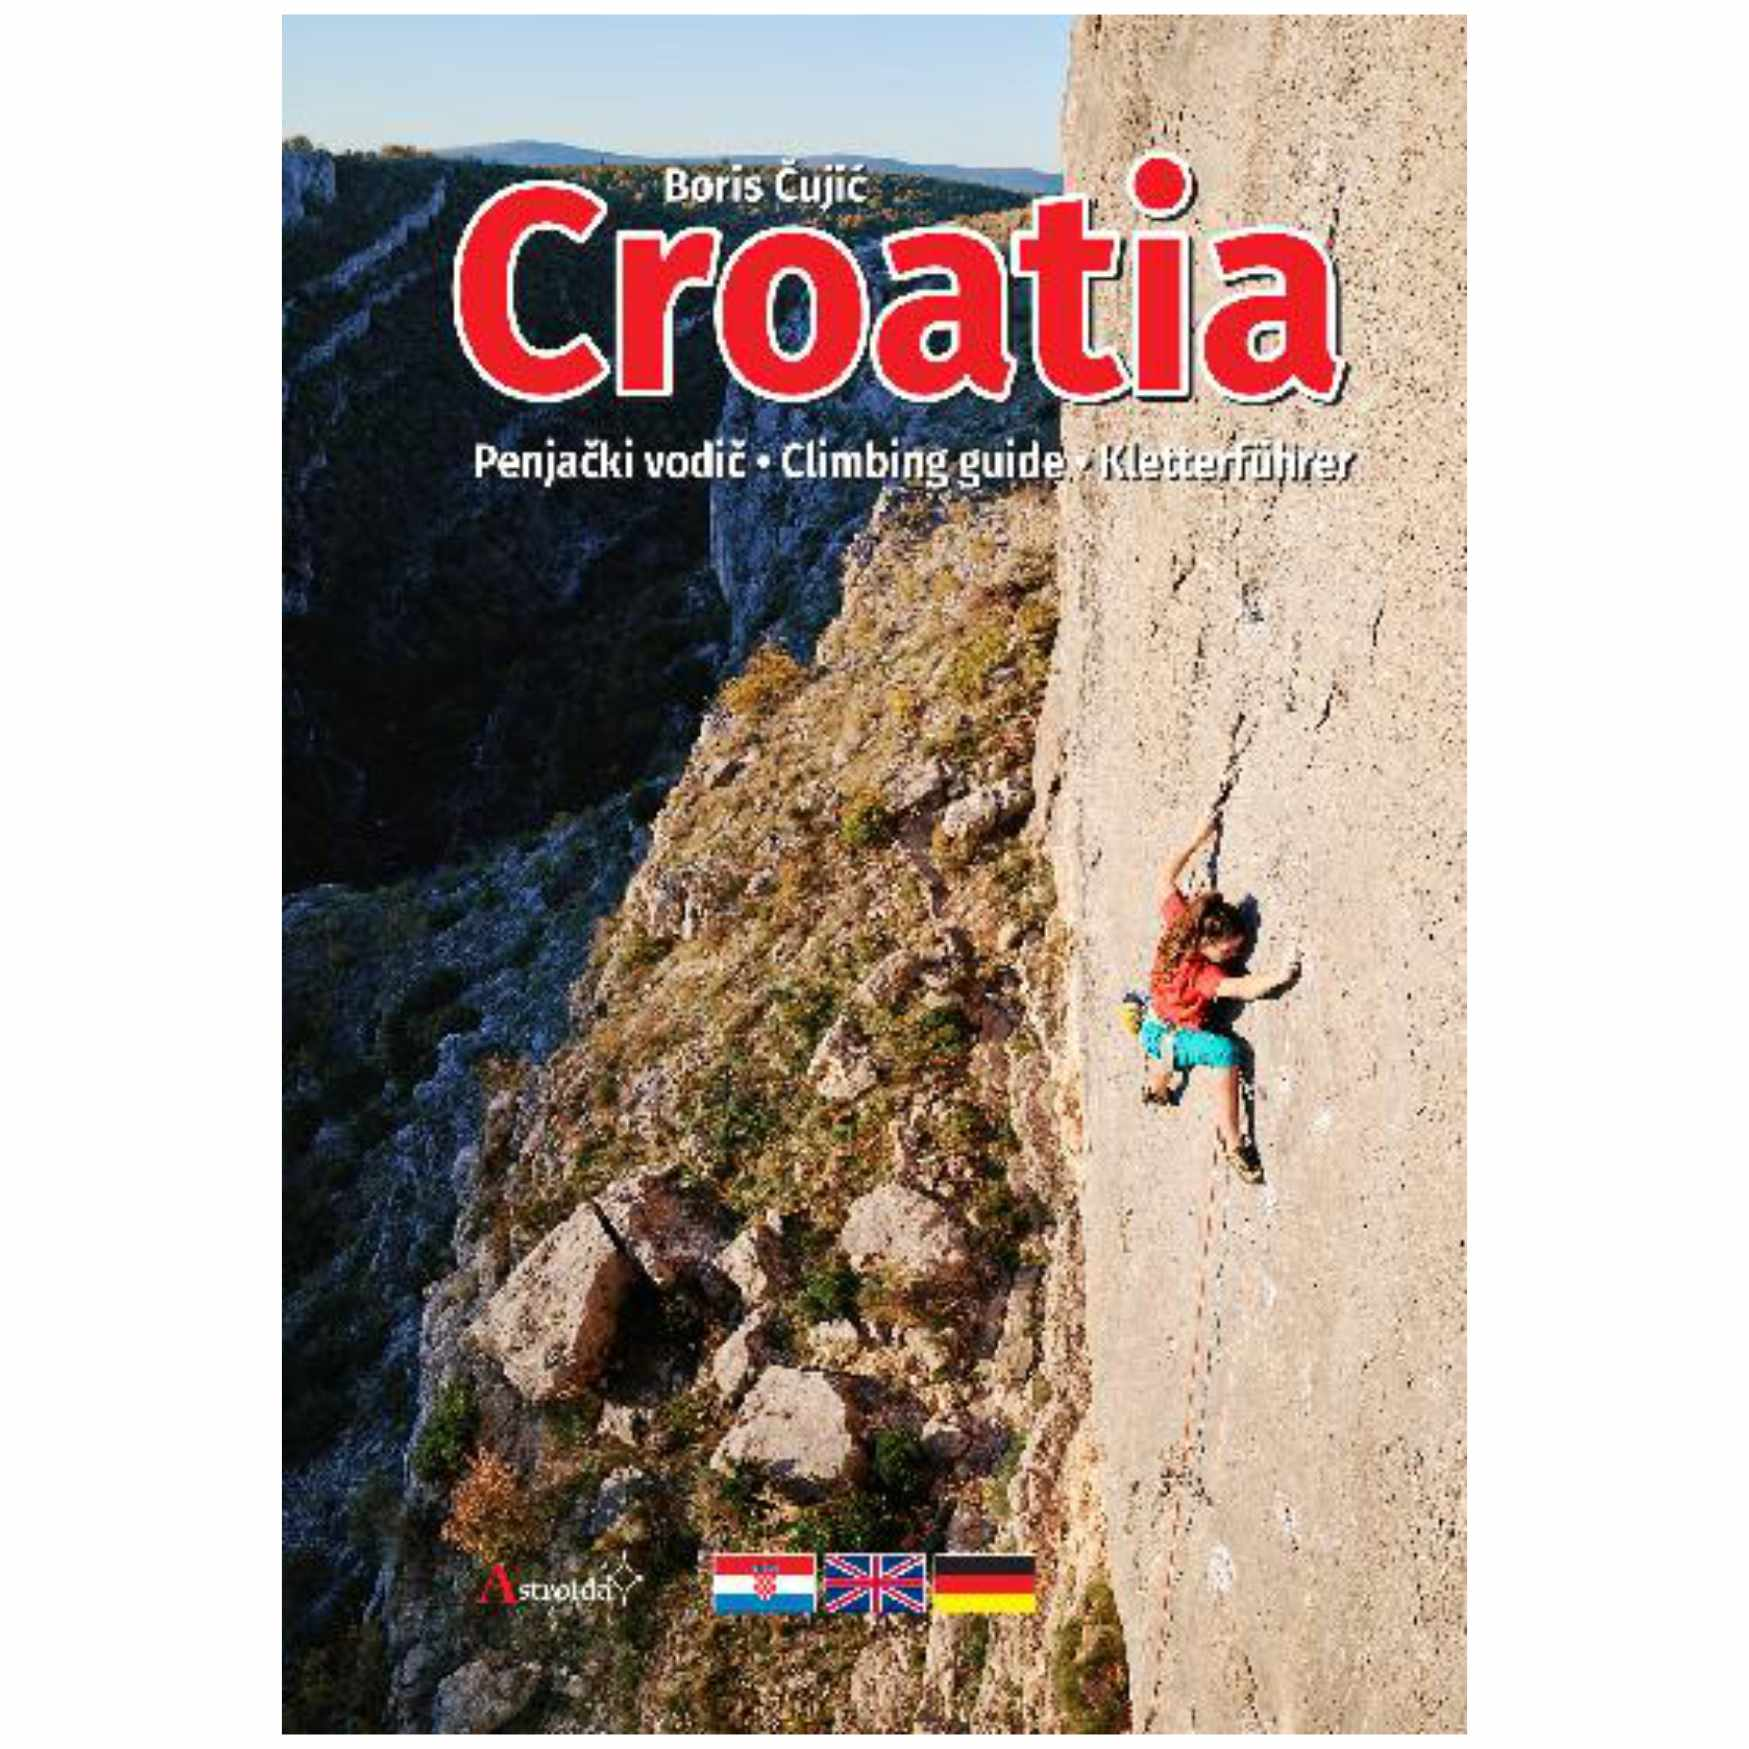
\includegraphics[width=0.8\textwidth]{images/uvod/tradicionalni_vodic.jpg}
    \caption{Prikaz tiskanog penjačkog vodiča}
\end{figure} 
\section{Ograničenja postojećih digitalnih alata}

S pojavom interneta i pametnih telefona, razvile su se digitalne platforme i mobilne aplikacije koje su djelomično riješile problem dostupnosti i ažurnosti podataka. One omogućuju centralizirano prikupljanje informacija, korisničke komentare i lakšu pretragu. Osim toga, nude i napredne funkcionalnosti poput vođenja osobnog dnevnika uspona, analize statistike, praćenja napretka i povezivanja s drugim penjačima.
Unatoč tim prednostima, digitalna rješenja nisu bez nedostataka. Većina postojećih aplikacija i dalje se oslanja na prikazivanje statičnih, dvodimenzionalnih \textit{topo} skica, čime se ne rješava temeljni problem identifikacije smjera u stvarnom okruženju. Nadalje, oslanjanje na elektronički uređaj u često udaljenim prirodnim okruženjima uvodi i praktične izazove. Ograničeno trajanje baterije i čest nedostatak mobilnog signala ili internetske veze mogu učiniti digitalne alate nedostupnima u trenutku kada su potrebni. Korisnik se tako suočava s dva ključna problema: interpretacija 2D prikaza i ovisnost o bateriji i signalu.

\begin{figure}[H]
    \centering
    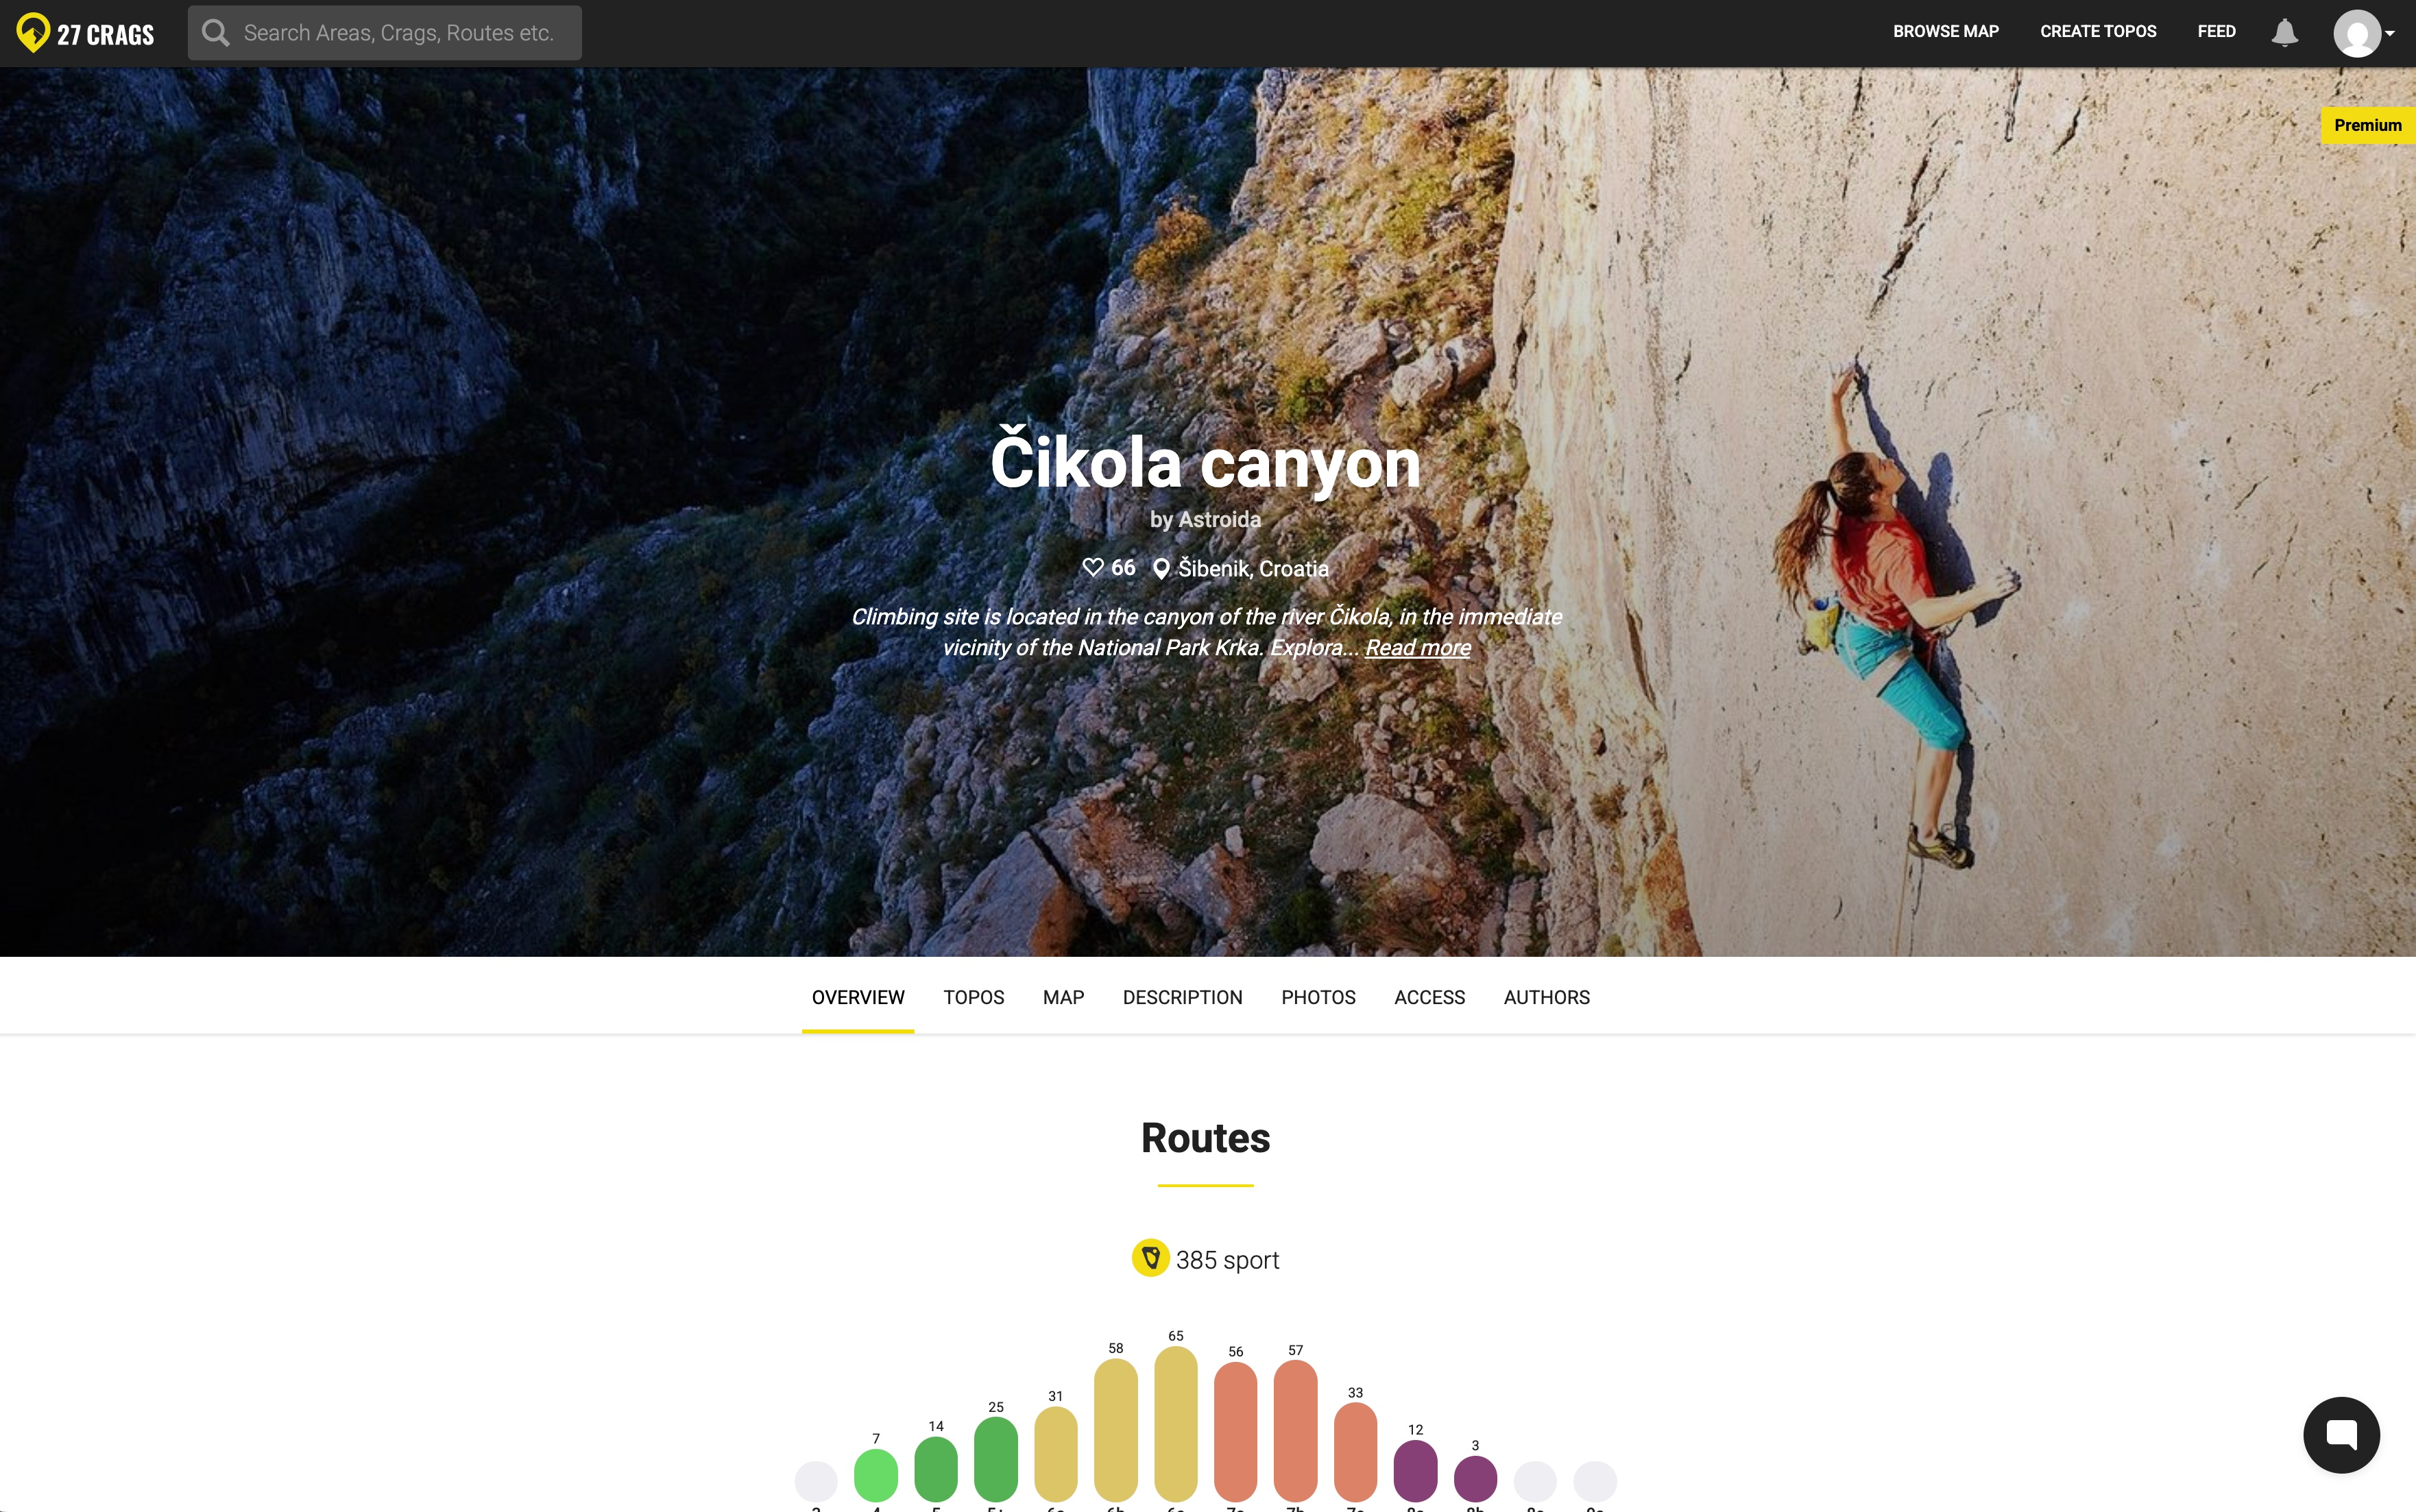
\includegraphics[width=0.75\textwidth]{images/uvod/27crags_cikola.jpeg}
    \caption{Prikaz penjačke lokacije Čikola na platformi 27crags}
\end{figure}

\section{Cilj i doprinos rada}

Navedeni nedostaci postojećih alata stvaraju potrebu za rješenjem koje pokriva njihove nedostatke. Cilj je iskoristiti mobilnu tehnologiju kako bi se stvorilo rješenje koje bi minimiziralo navedene nedostatke. Ideja je omogućiti penjačima da jednostavnim usmjeravanjem kamere mobilnog uređaja prema stijeni dobije vizualnu informaciju o položaju i nazivima smjerova izravno u stvarnom okruženju korištenjem tehnologije proširene stvarnosti. Takav pristup ne samo da štedi vrijeme i smanjuje frustracije, već i omogućuje sigurnije iskustvo penjanja. 
